\documentclass[10pt,letterpaper]{article}
\usepackage[utf8]{inputenc}
\usepackage[spanish]{babel}
\usepackage{amsmath}
\usepackage{amsfonts}
\usepackage{amssymb}
\usepackage{graphicx}
\usepackage{float}

\graphicspath{ {img/} } 

\author{David Alejandro Castillo Chíquiza,\\ Juan Sebastián Ruiz Bulla,\\ Juan Pablo Ortiz Rubio}
\title{Taller 3}

\begin{document}

\maketitle

\section{Punto Silueta "Picasso"}

	\subsection{Enunciado}
	Reconstruir el perfil superior e inferior ("Silueta") de picasso.
	\begin{figure}[H]
		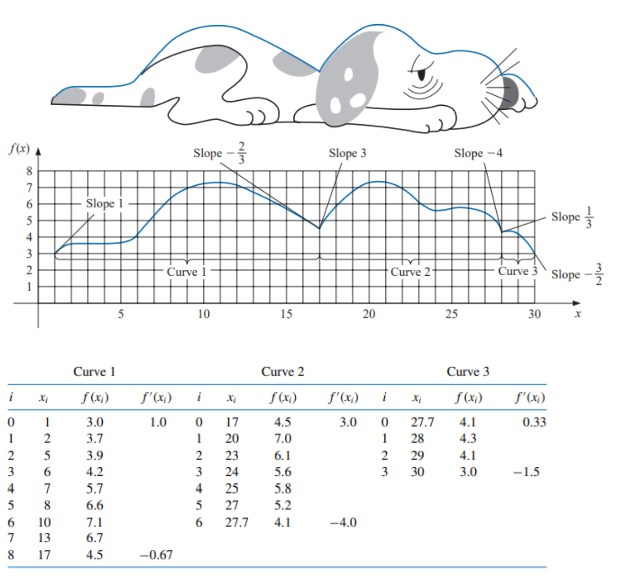
\includegraphics[scale=0.5]{EnunciadoSilueta}
		\centering
		\caption{Silueta dada en el enunciado.}
		\centering
	\end{figure}

	\subsection{Solución}
	Para este punto realizamos 2 soluciones en 2 lenguajes diferentes(Python y R), esencialmente la solución propuesta es la misma en las dos opciones presentadas, la diferencia radica principalmente en la facilidad que presenta el lenguaje R para realizar la interpolación en las curvas, en comparación en el lenguaje Python es ligeramente mas largo y tedioso el realizar esto, sin embargo, eso no quiere decir que sea mas difícil o complejo de realizar en este lenguaje.\\
	
	El funcionamiento de ambas opciones consiste en hacer uso de arreglos cuyos valores son algunos de los puntos en $x$ y $y$ que conforman la silueta del perrito, luego estos puntos son pasados por funciones brindadas por el mismo lenguaje o por librerías externas al lenguaje base, cabe resaltar que no se pasan todos los puntos de una sola vez, en cambio se va realizando por curvas, para conseguir un mejor resultado al momento de que se realicen las gráficas, el método para interpolar en Pythion fue el cubico, por otro lado en R utilizamos fmm conocido como Forsythe, Malcom y Moler (el cual es un metodo cubico exacto que se ajusta por medio de 4 puntos a los extremos de los  datos para determinar las condiciones finales).\\
	
	\begin{figure}[H]
		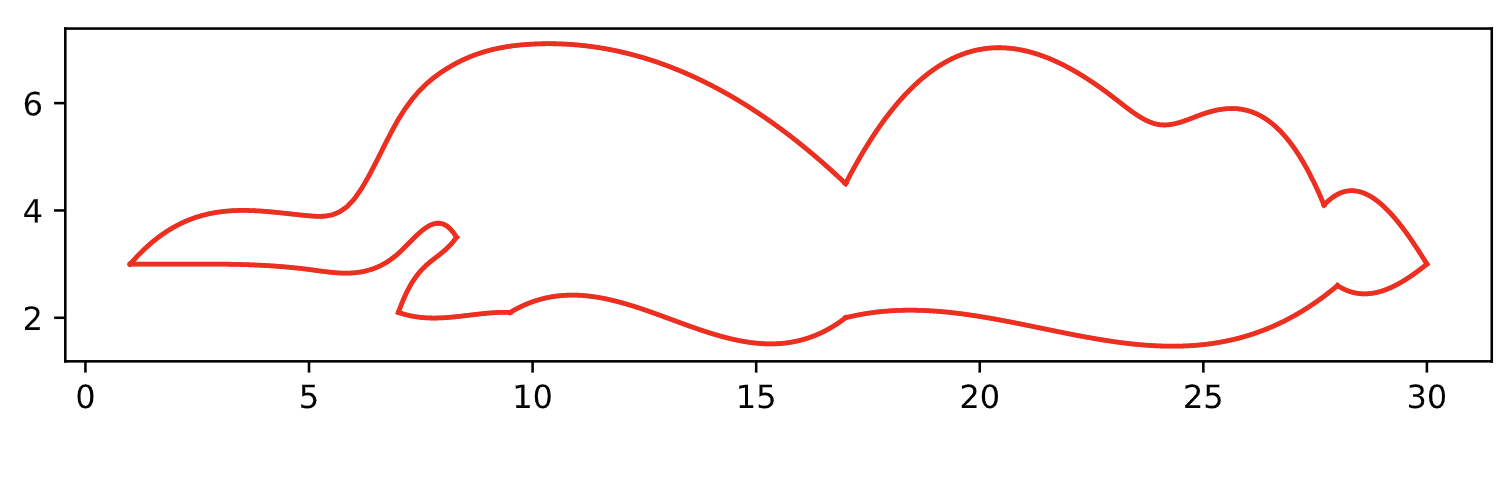
\includegraphics[width=\textwidth]{PerroSinPuntos}
		\caption{Silueta generada en Python.}
		\centering
	\end{figure}
	
	\begin{figure}[H]
		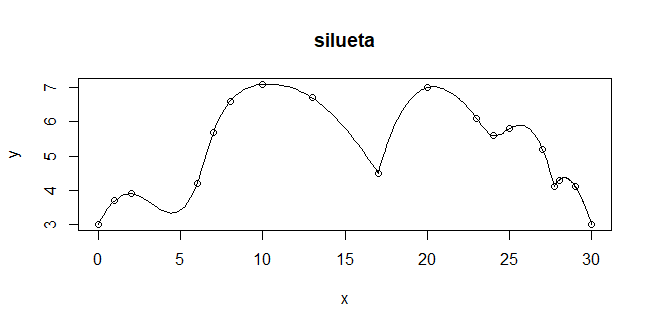
\includegraphics[width=\textwidth]{Rplot}
		\caption{Silueta generada en R.}
		\centering
	\end{figure}
	
\section{Punto 13}
	
	\subsection{Enunciado}
	Escala de gravamen del Impuesto a la renta.\\
	\begin{center}
		\begin{tabular}{|c|c|c|}
			\hline
			Base imponible & Cuota Integra & Tipo\\ \hline
			$4.410.000$ & $1.165.978$ & $38,86\%$ \\ 
			$4.830.000$ & $1.329.190$ & $41,02\%$ \\
			$5.250.000$ & $1.501.474$ & $43,18\%$ \\
			$5.670.000$ & $1.682.830$ &			  \\ \hline
		\end{tabular}
	\end{center}
	La cuota íntegra del Impuesto sobre la Renta se determina aplicando una fórmula basada en la interpolación lineal. Un contribuyente tiene una base imponible de 5 millones. Para calcular lo que tiene que pagar a Hacienda efectúa las siguientes operaciones, consultando la escala de gravamen anterior:\\
	\begin{center}
		\begin{tabular}{c c c c}
			Base & $5.000.000$& & Cuota \\
			Hasta & $4.830.000$& & $1.329.190$ \\
			Resto & $170.000$ & al $41,02\%$ & $69.734$\\
				  & 		  & Suma & $1.398.924$
		\end{tabular}
	\end{center} 
	El tipo marginal del $41,02\%$ que aparece en la escala de gravamen es precisamente el cociente de las diferencias entre las cuotas íntegras y las bases imponibles más próximas en la escala a los 5 millones.
	$$\frac{1.501.474 - 1.329.190}{5.250.000 - 4.830.000}=0,4102$$ \\
	La  formula aplicada en definitiva es,
	$$Cuota=1.329.190 + 0,4102(Base 4.830.000)$$\\
	Para las bases comprendidas en el intervalo [4.830.000,5.250.000].\\
	En particular, para una base imponible de $5.250.000$ es indiferente aplicar la fórmula anterior o tomar directamente el valor de la tabla. En términos matemáticos esto equivale a decir que la Cuota es una función continua de la Base imponible. El Impuesto sobre la Renta es progresivo, es decir, que el tipo de la imposición aumenta con la base imponible, como se comprueba observando la escala de gravamen. Así, el tipo medio correspondiente a $4.830.000$ es el $27,52\%$ y el de $5.250.000$ es el $28,60\%$.\\\\
	El contribuyente se siente perjudicado por el hecho de que al Resto de su Base imponible (170.000) se le aplica el mismo tipo marginal $(41,02\%)$ que, a otro contribuyente con una Base de 5.250.000, alegando que debe aplicársele el correspondiente a la base más próxima en la escala $(4.830.000)$ que es del $38,86$. Hacienda, por su parte, rechaza estos argumentos y efectúa la liquidación según sus normas. El sujeto del impuesto interpone recurso (tutela) ante el Tribunal competente, que considera en parte sus alegaciones. El fallo establece que en todo caso se debería aplicar un tipo marginal intermedio.\\\\
	Como experto en temas fiscales debes elaborar un informe para que Hacienda conozca las diferencias entre el actual sistema impositivo y los posibles métodos de determinar la imposición correspondiente a la base de 5 millones por interpolación de segundo y tercer grado en la escala de gravamen. ¿En cada grado debe añadirse la base más próxima a 5 millones?	
	\subsection{Solución}
	Para la solución de este problema realizamos una implementación en Python (Jupiter Notebook), para realizar esto fue necesario importar una librería que fuese capaz de realizar interpolaciones, el funcionamiento de esta solución consiste que recibir los datos dados en el , con estos se calcula por medio de splines lineales, cuadráticos y cúbicos el tipo y la cuota integra según corresponda todo esto calculado con la base imponible de $5'000.000$.\\
	
	\begin{figure}[H]
		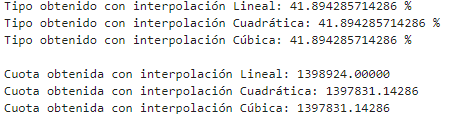
\includegraphics[width=\textwidth]{Results}
		\caption{Resultados.}
		\centering
	\end{figure}	
	Dados los resultados aparentemente no existe una diferencia significativa entre las interpolaciones cuadráticas y cubicas, por el contrario las 2 anteriores si se diferencian significativamente de la lineal, con esto podemos decir que cualquiera de las interpolaciones, ya sea cuadrática o cubica son mejores a la original, ya que nos dan una cuota integra más alta a la que originalmente se  tenia. \\
	\begin{figure}[H]
		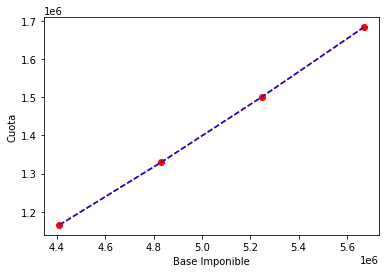
\includegraphics[width=\textwidth]{Grafica13}
		\caption{Relación base imponible y cuota integra.}
		\centering
	\end{figure}
	Finalmente con la gráfica anterior podemos apreciar que un aumento en la base imponible genera un crecimiento linealmente proporcional al valor.   
	
\end{document}